\chapter{appendices} \label{appA}

\section{Conference Publication, and Presentation for proposed investigations}


\subsection{OCI Investigations}

Copper Moutian

M\&C 2023

\subsection{Hybrid-Delta Tracking Schemes}

M\&C 2023

\subsection{Acceleration and Abstraction of Python}

SciPy 2024

S3C 2024

Monte Carlo Computational Summit

M\&C 2023

ANS Annual 2022

SciPy 2022

\section{All Publications}

\section{Submitted Draft: Performant and Portable\\ Monte Carlo Neutron Transport via Numba}
\label{app:cise}

This paper was submitted to \textit{IEEE Computing in Science and Engineering} on September 3rd 2024. 
I have not received a response.
A preprint was posted to arxiv and has been the assigned the DOI 10.48550/arXiv.2409.04668.

My coauthors are all members of the Center for Exascale Monte Carlo Neutron Transport (CEMeNT) includes
\begin{itemize}
    \item Ilham Variansyah, PhD (committee member)
    \item Braxton Cuneo, PhD
    \item Todd S. Palmer, PhD (committee member)
    \item Kyle E. Niemeyer, PhD (advisor)
\end{itemize}
As MC/DC is the primary deliverable of CEMeNT it is a deeply combative effort.


%\subsection{My work}
%I was the primary author and as such drafted the whole paper.
%I received significant edits from all my co authors who all contributed to the work.
%I collected the data

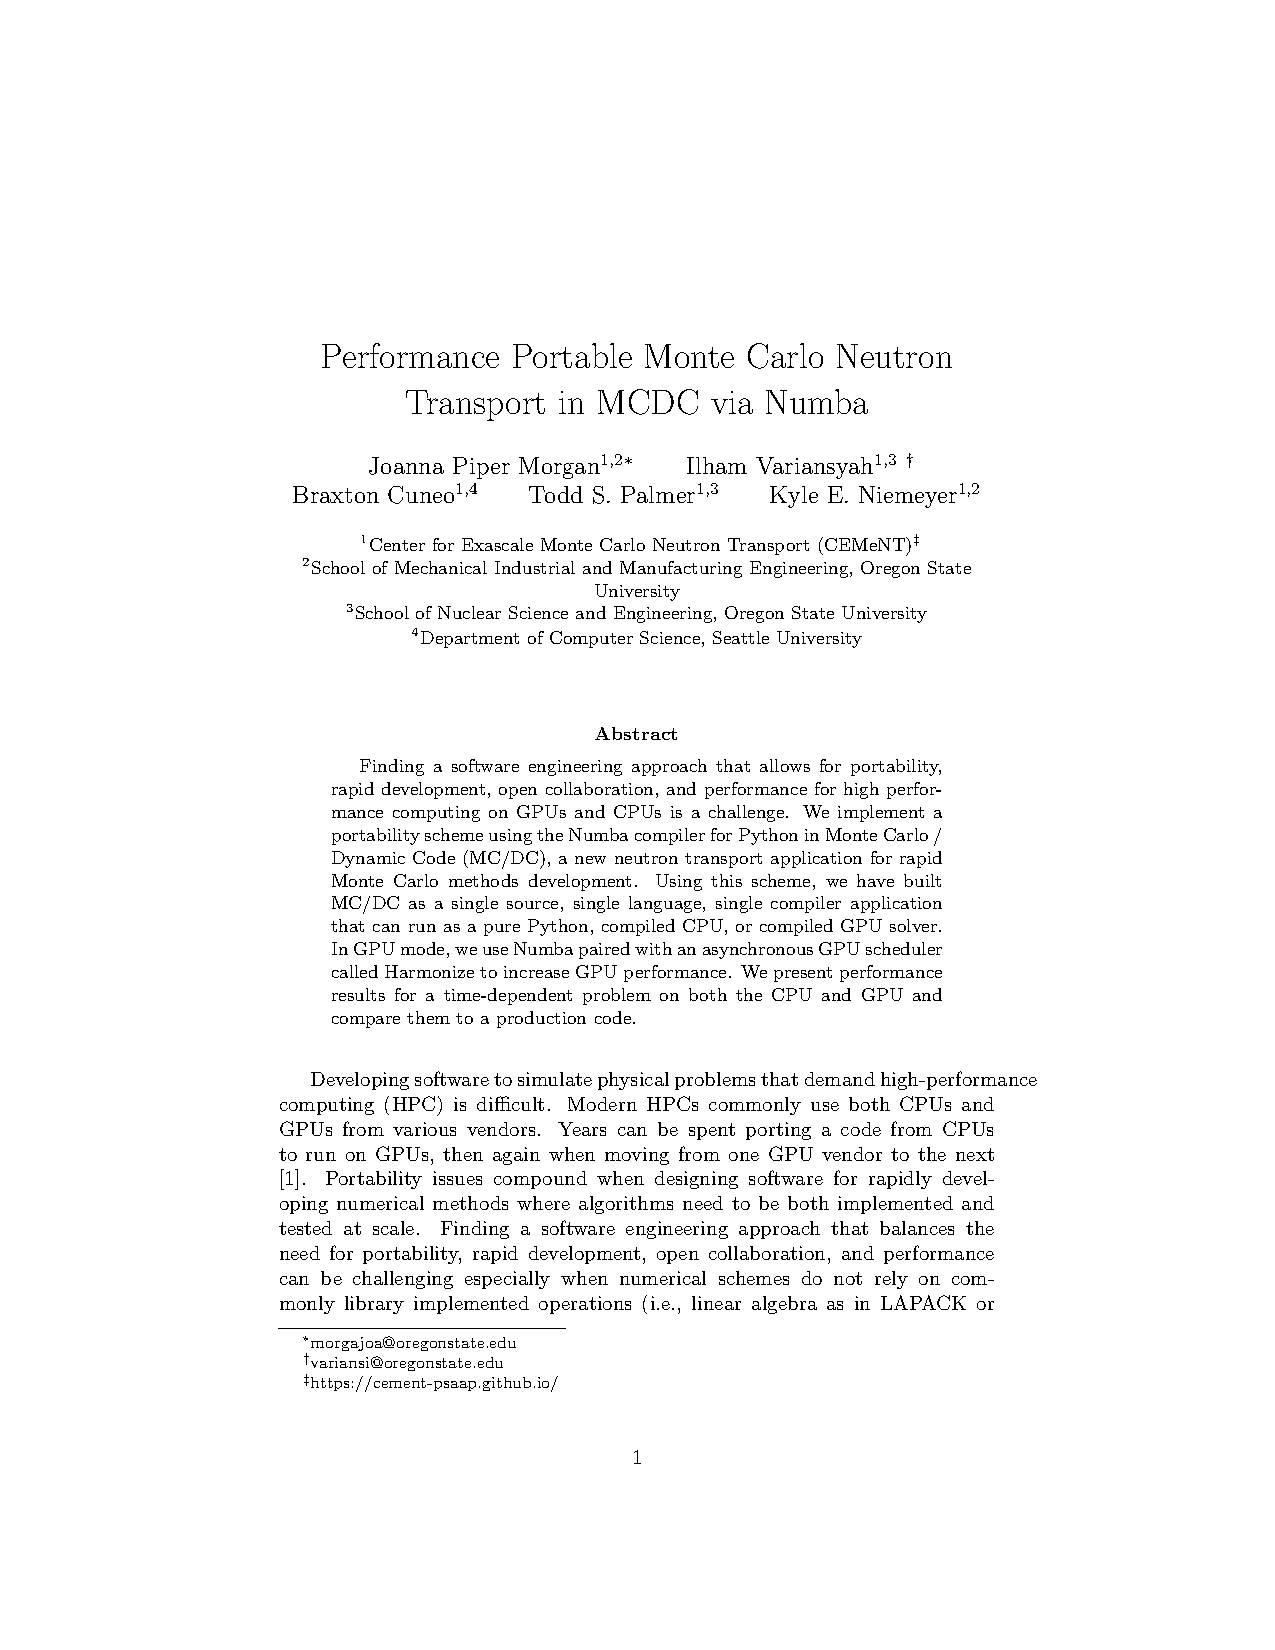
\includepdf[pages=-]{appendix/ana_numba_mcdc.pdf}


\section{Hybrid-Delta Tracking on a Structured Mesh in MCATK}

This work was submitted to, accepted with mino

\begin{itemize}
    \item Travis J. Trahan, PhD
    \item Timothy P. Burke, PhD
    \item Collin J. Josey, PhD
    \item Kyle E. Niemeyer, PhD
\end{itemize}

\label{app:hybridmcatk}
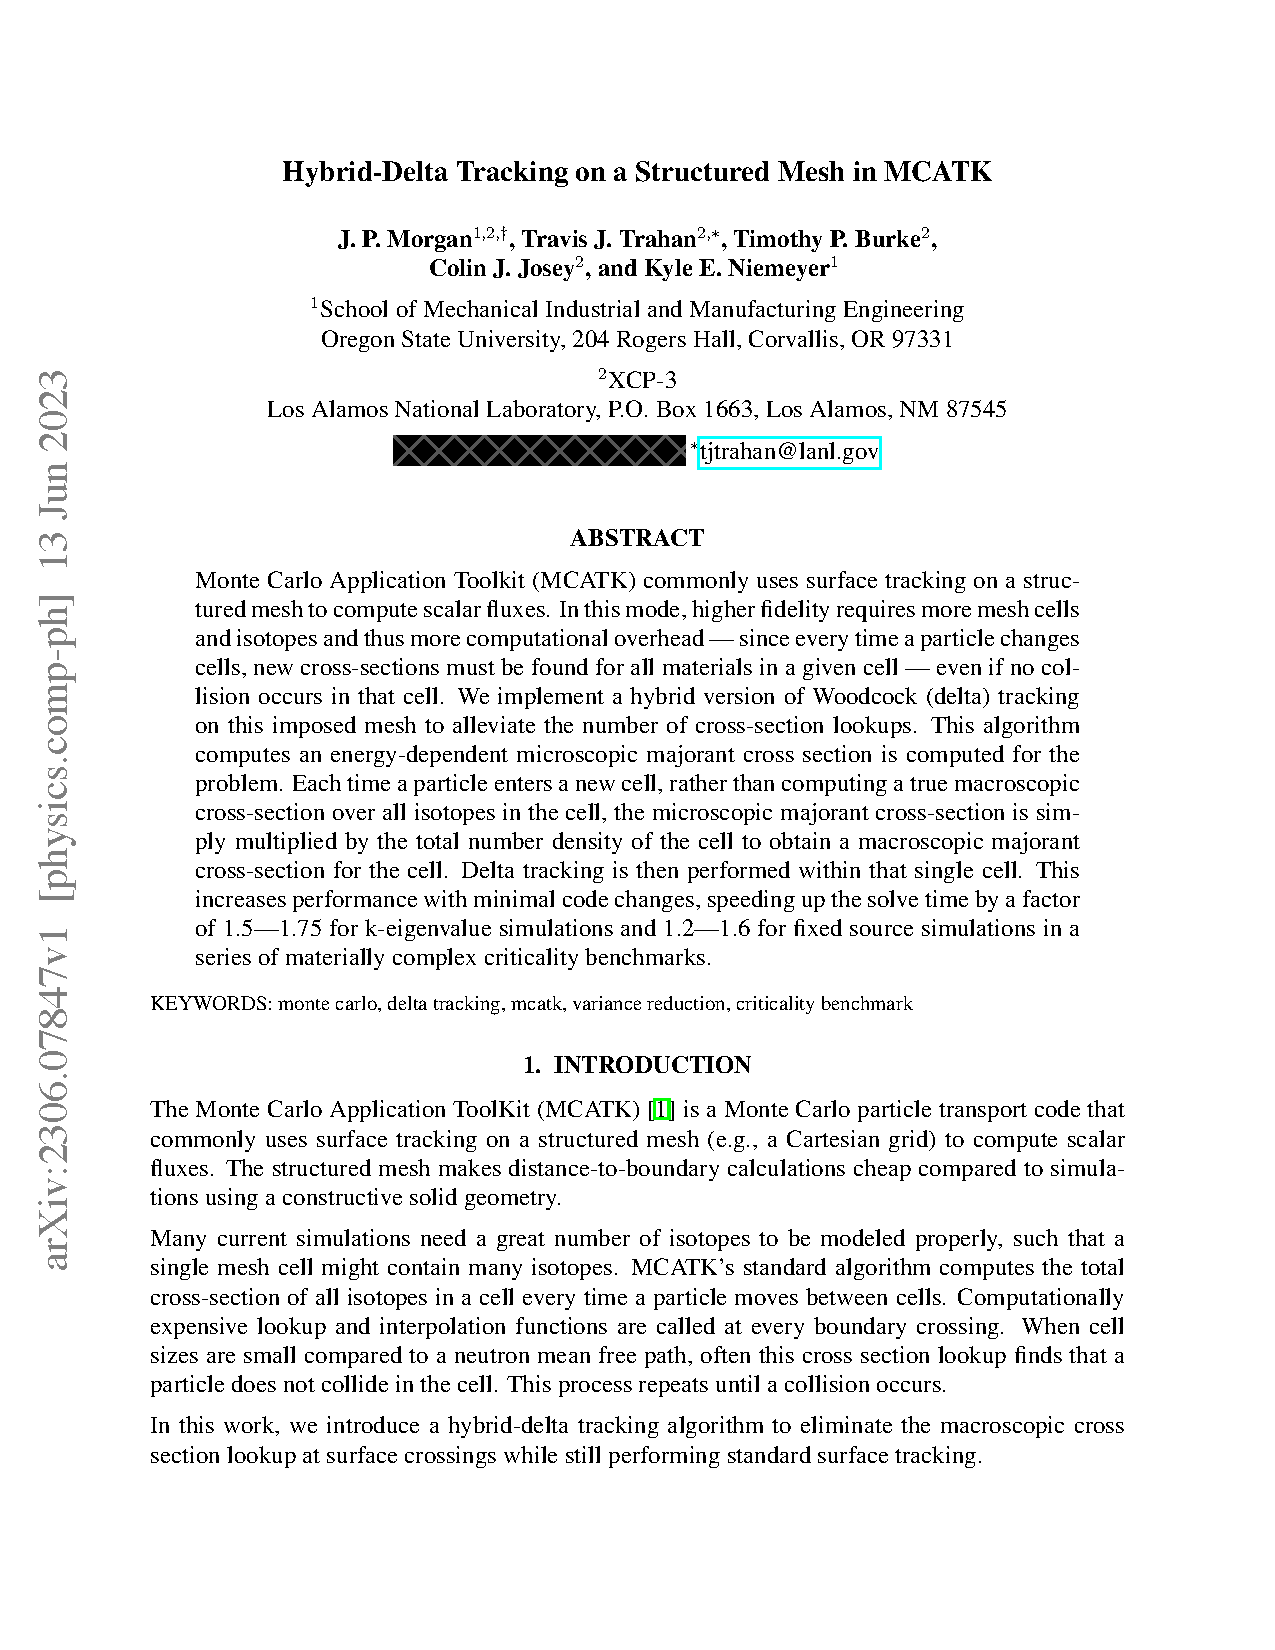
\includepdf[pages=-]{appendix/delta_tracking_mcatk.pdf}

\section{Draft: Therefore paper}
\label{app:therefore}
%\includepdf[pages=-]{ANS2022Clements.pdf}
%\includepdf[pages=-]{OlsonANSWinter2022.pdf}
%\includepdf[pages=-]{journal_draft.pdf}


